% Imporditud: tools/import_eksperimendid.py
% Allikas: Eesti füüsikaolümpiaadi eksperimendi ülesannete
%   kogu (Rael Kalda, 2023), ülesanne Ü175, lahendus L175.
\setAuthor{Eero Uustalu}
\setRound{piirkonnavoor}
\setYear{2018}
\setNumber{G E2}
\setDifficulty{5}
\setTopic{geomeetriline optika}
\setVahendid{keeduklaas veega, millimeeterpaber, paberteip, käärid}
\setPunktid{12}
\setAllikas{Eksperimendi kogu Ü175, lahendus lk 133}
\setLahendusseis{kasitsi}

\prob{Murdumisnäitaja}
Määrake võimalikult täpselt vee murdumisnäitaja $n_{\text{vesi}}$.

\begin{center}
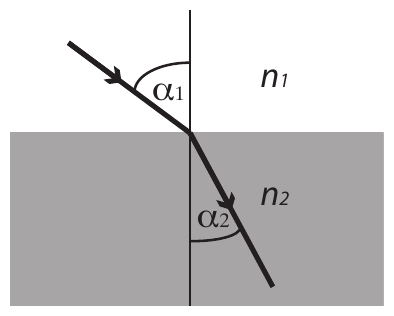
\includegraphics[width=0.30\linewidth]{2018-v2g-ge2-yl.png}
\end{center}

\textit{Vihje:} Murdumisseadus kahe keskkonna piirpinnal avaldub kujul
$n_1\sin\alpha_1 = n_2\sin\alpha_2$.

\hint

\solu
\textit{Lahendus on kogumikus lk 133. Siia ei ole seda veel ümber kirjutatud, sest originaalis on tabel või joonis, mis PDF-i tekstikihist loetavalt välja ei tule.}
\probend
